% \documentclass[8pt]{article}
\documentclass[8pt]{extarticle}

\usepackage[a2paper, total={13in, 17in}]{geometry}

\usepackage{graphicx}
\usepackage{titling}

\pagenumbering{gobble}

\setlength{\droptitle}{-15em}

\title{AI Fix Roads SU Data School Hackathon}
\author{Jan Dalhuysen \and Hugo Bruwer \and Nathan Sparg \and Dannike Zietsman \and Joseph Carmody}
\date{}

\begin{document}

\maketitle

\vspace{5px}

\begin{center}
\textbf{Note:} PDF is a vector format. Zoom in to see small details better.
\end{center}

\vspace{10px}

\section{Introduction}

\textbf{Challenge:} Predict the amount of asphalt required to fill a pothole given just an image of that pothole? \\
\textbf{Bonus:} How might you commercialise this model? How can your model be used practically in industry?

\section{Detecting Stick length}

\textbf{Disjoint-set data structure} \\

\noindent Invented 1964 by Bernard A. Galler and Michael J. Fischer

\noindent In computer science, a disjoint-set data structure, also called a union-find data structure or merge-find set, is a data structure that stores a collection of disjoint (non-overlapping) sets. Equivalently, it stores a partition of a set into disjoint subsets. It provides operations for adding new sets, merging sets (replacing them by their union), and finding a representative member of a set. The last operation makes it possible to find out efficiently if any two elements are in the same or different sets. -Wikipedia

\noindent For detecting the length of the stick in the image, the disjoint-set algorithm was used. The algorithm was implemented in Python using the \textbf{scikit-image} library, that modified the image to only display the red pixels in the image. The DSU then groups red pixels together, while discarding other clutter, like red pixels that don't form part of the red paint on the stick.

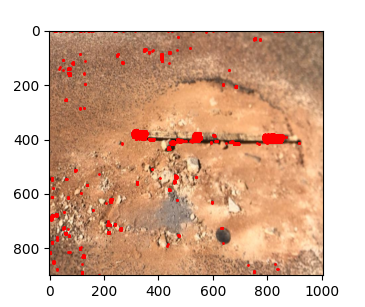
\includegraphics[width=0.30\columnwidth]{pdf_image_1.png}
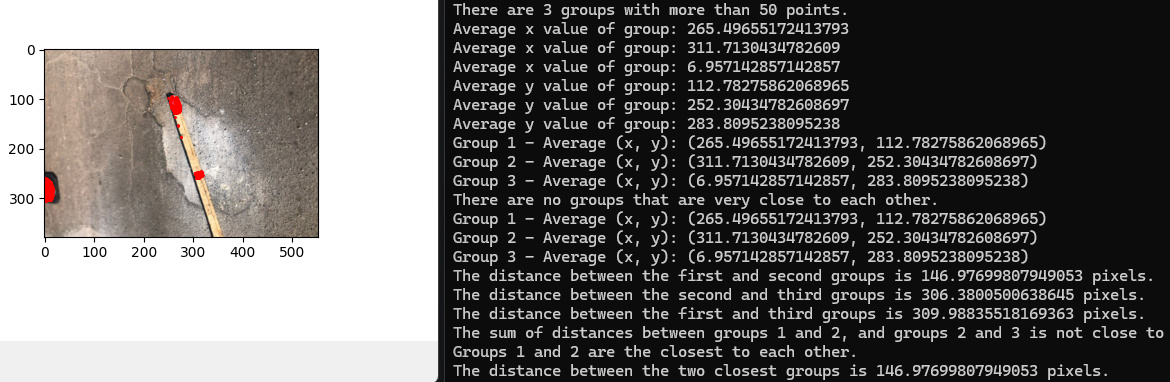
\includegraphics[width=0.70\columnwidth]{pdf_image_2.png}

\section{Detecting Pothole dimensions}

\vspace{10px}

% The pothole_yolov8_nano model by Hugging Face user sovitrath was initally used to detect the pothole in the image, however this model wasn't good enough to detect the dimensions of the pothole reliably.
The pothole yolov8 nano model by Hugging Face user sovitrath was initially used to detect the pothole in the image, however this model was not good enough to detect the dimensions of the pothole reliably.
The next step was then to use the base YoloV8 model from the ultralytics library and then train it on the pothole images and labels provided.
The training photos with their labels showing the bounding boxes of the potholes and the models improvement over time are clearly shown below.

\vspace{20px}

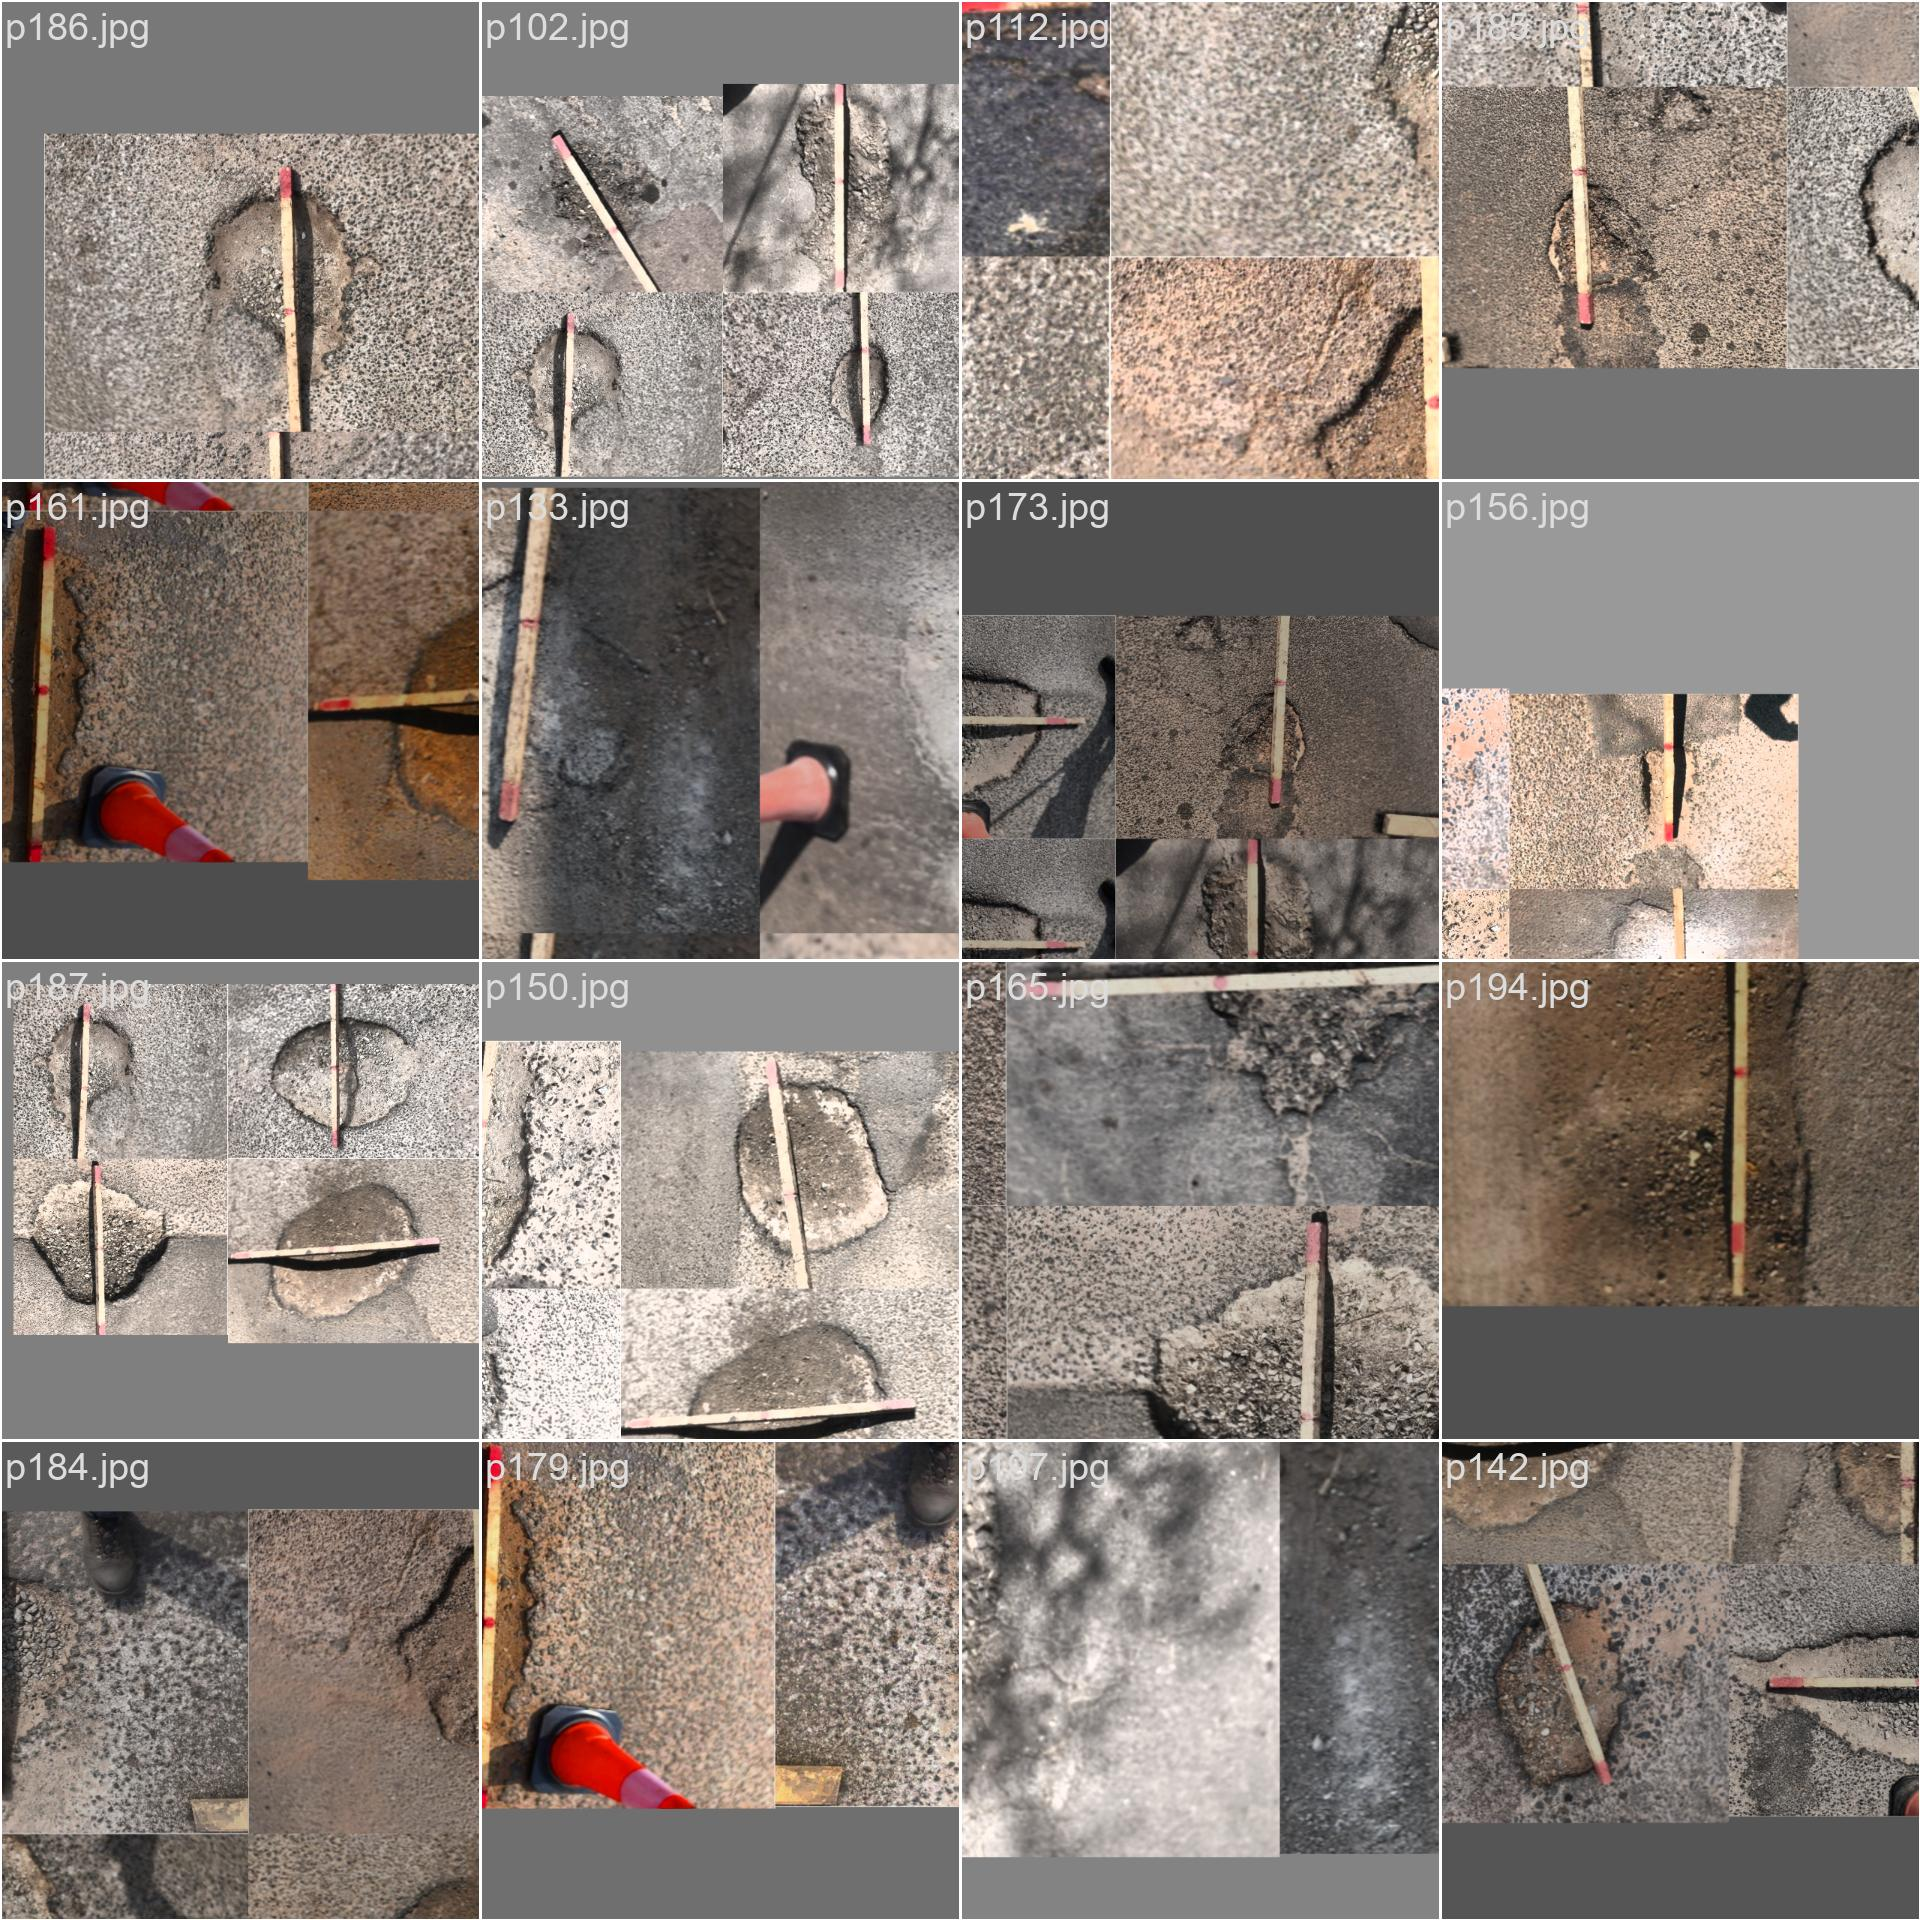
\includegraphics[width=0.30\columnwidth]{train_batch1.jpg}
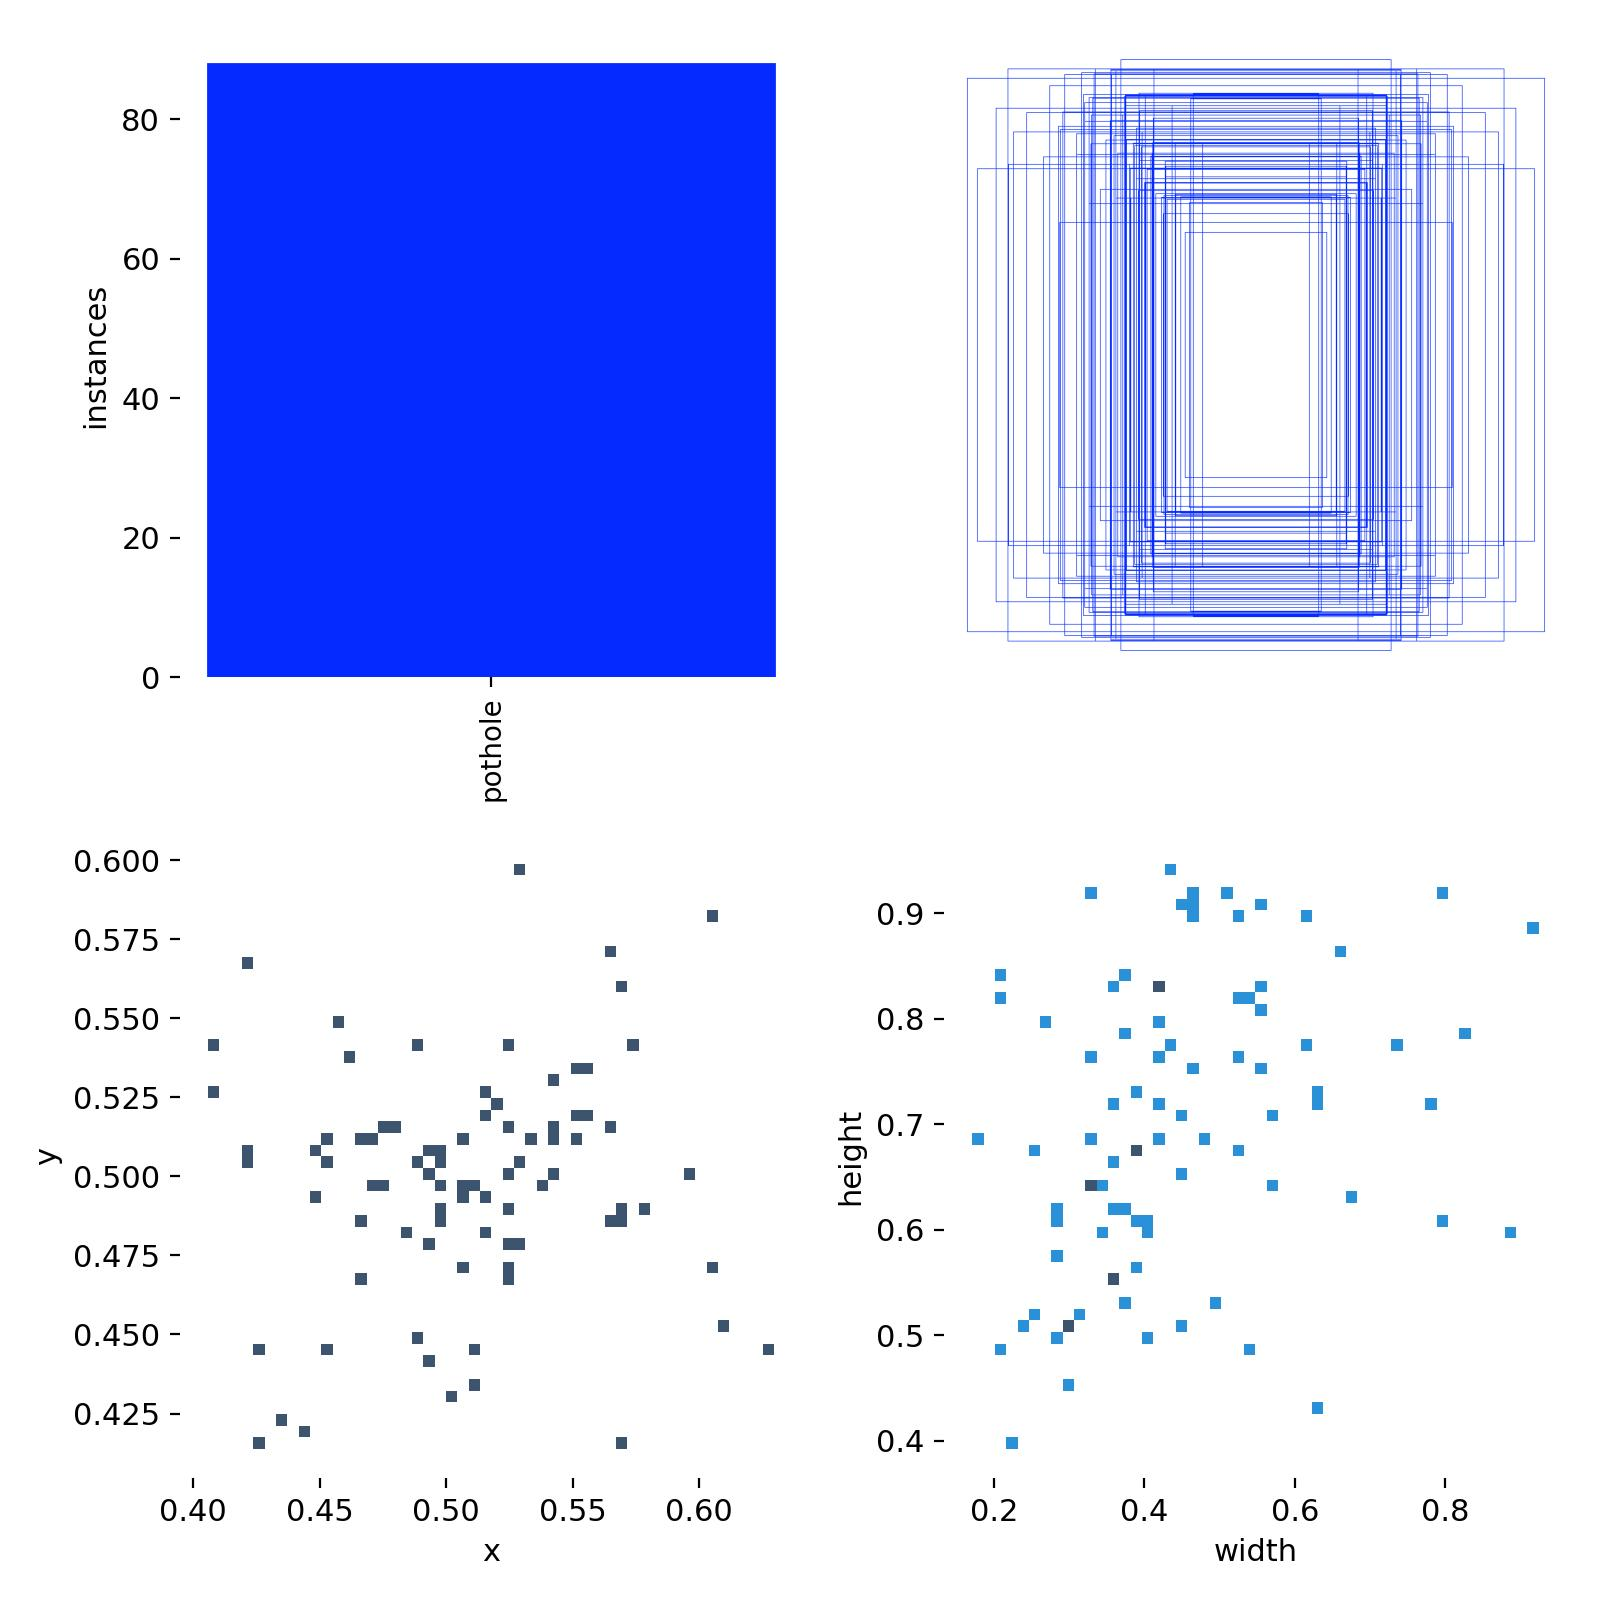
\includegraphics[width=0.30\columnwidth]{labels.jpg}
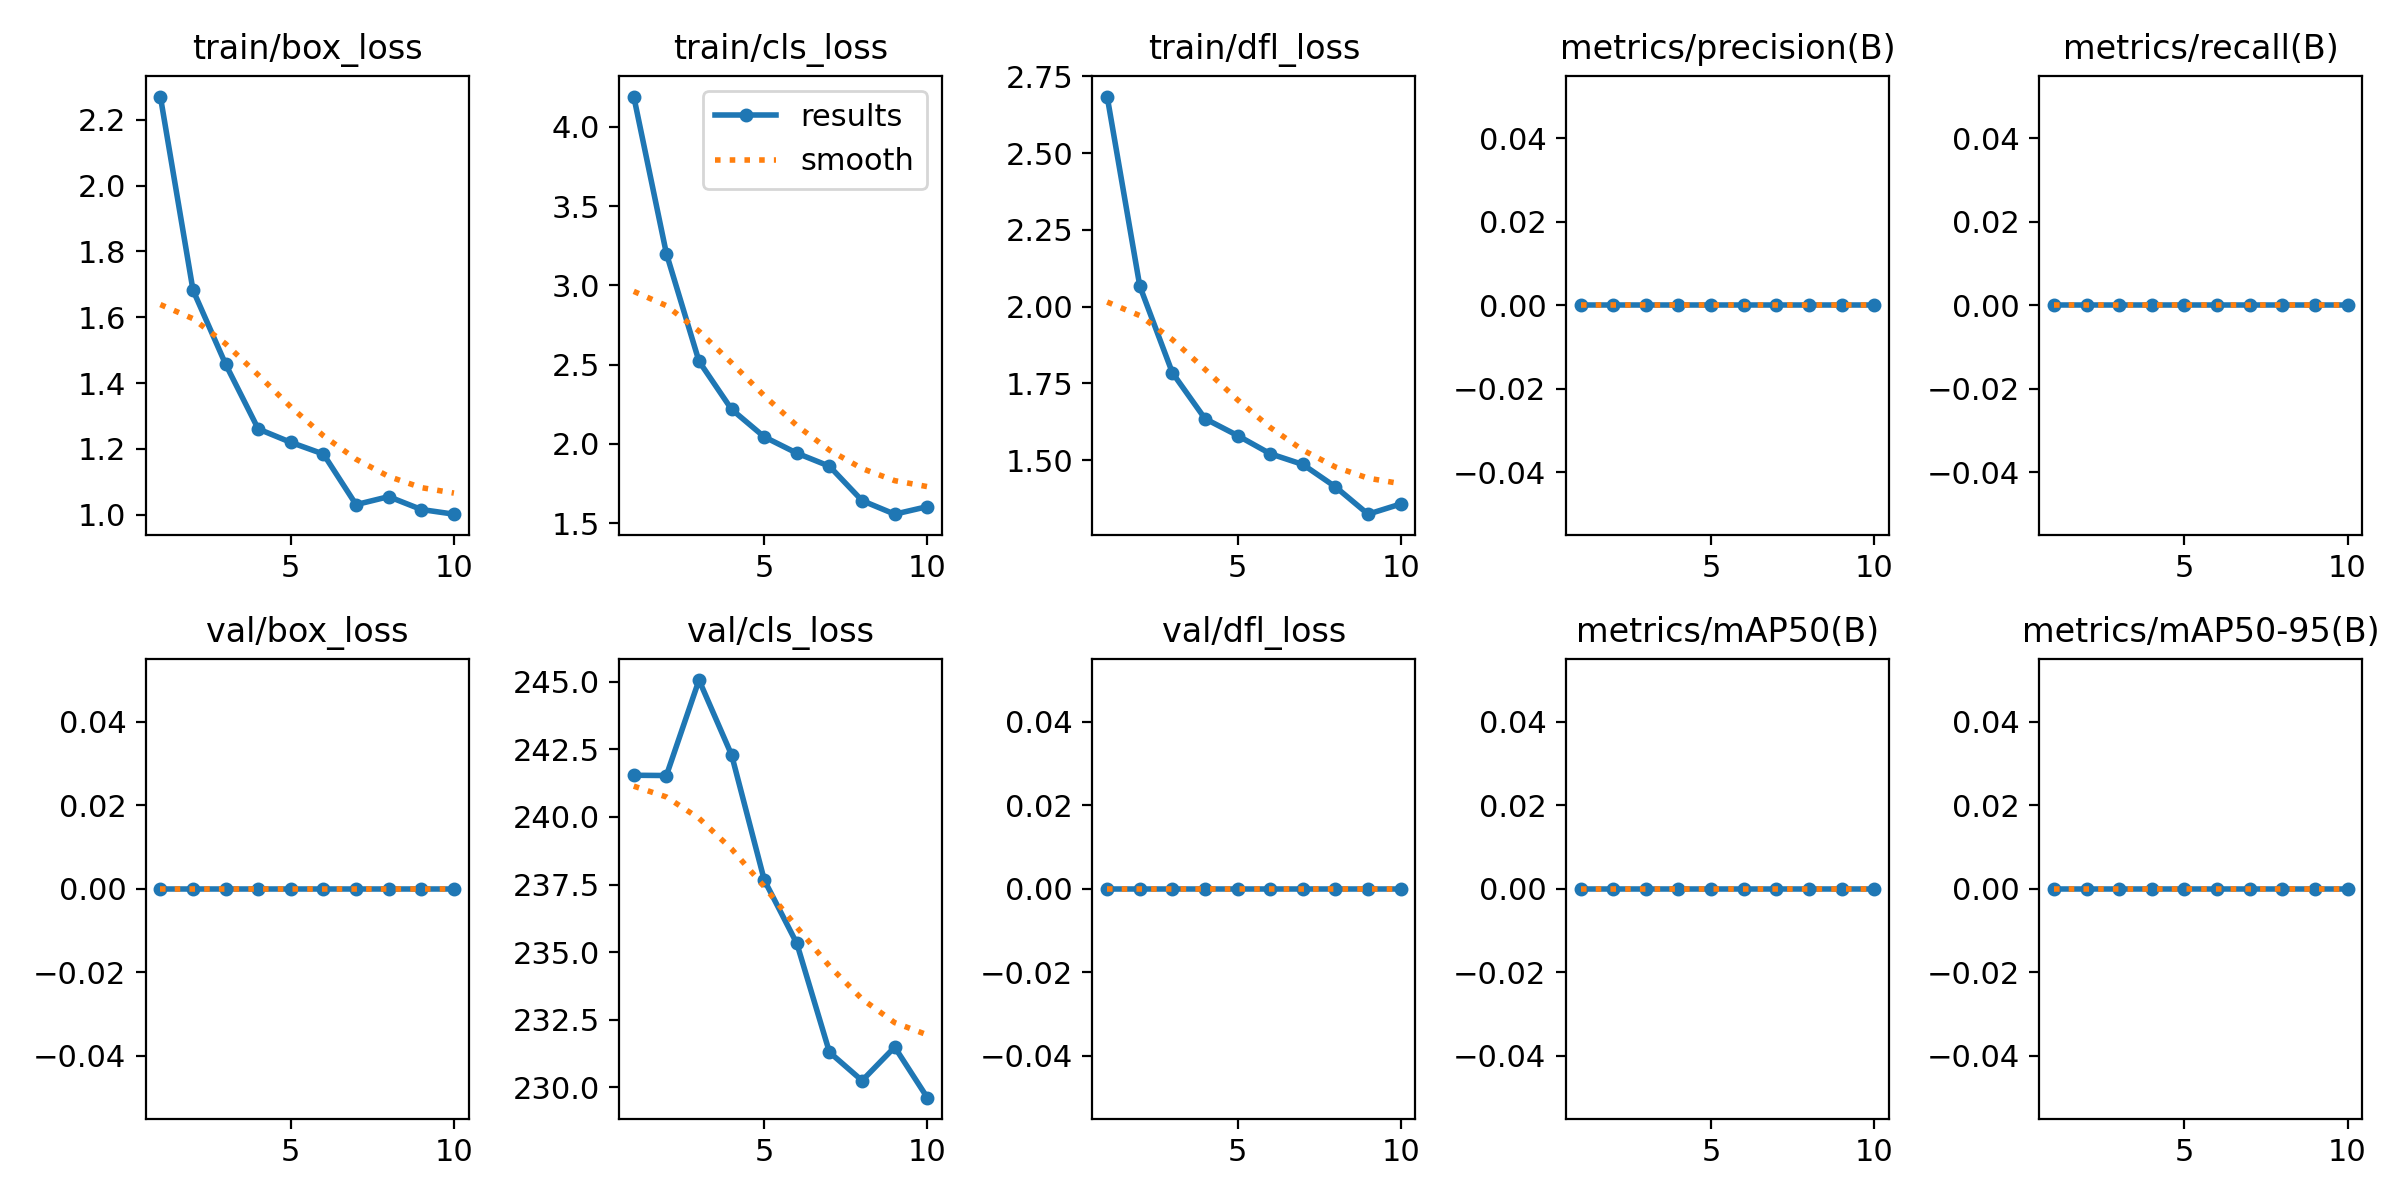
\includegraphics[width=0.40\columnwidth]{results.png}

\section{Predicting}

\vspace{10px}

To find the correlation between the area of the pothole and the number of bags of asphalt used that is needed to fill them the \textbf{scikit-learn LinearRegression} model was used. The model was trained on the data set that was provided and the plot below clearly shows the correlation between the two variables. As the area of the pothole increases so does the number of bags of asphalt needed to fill it. An example of the csv file used to train the model is also included below.

\vspace{20px}

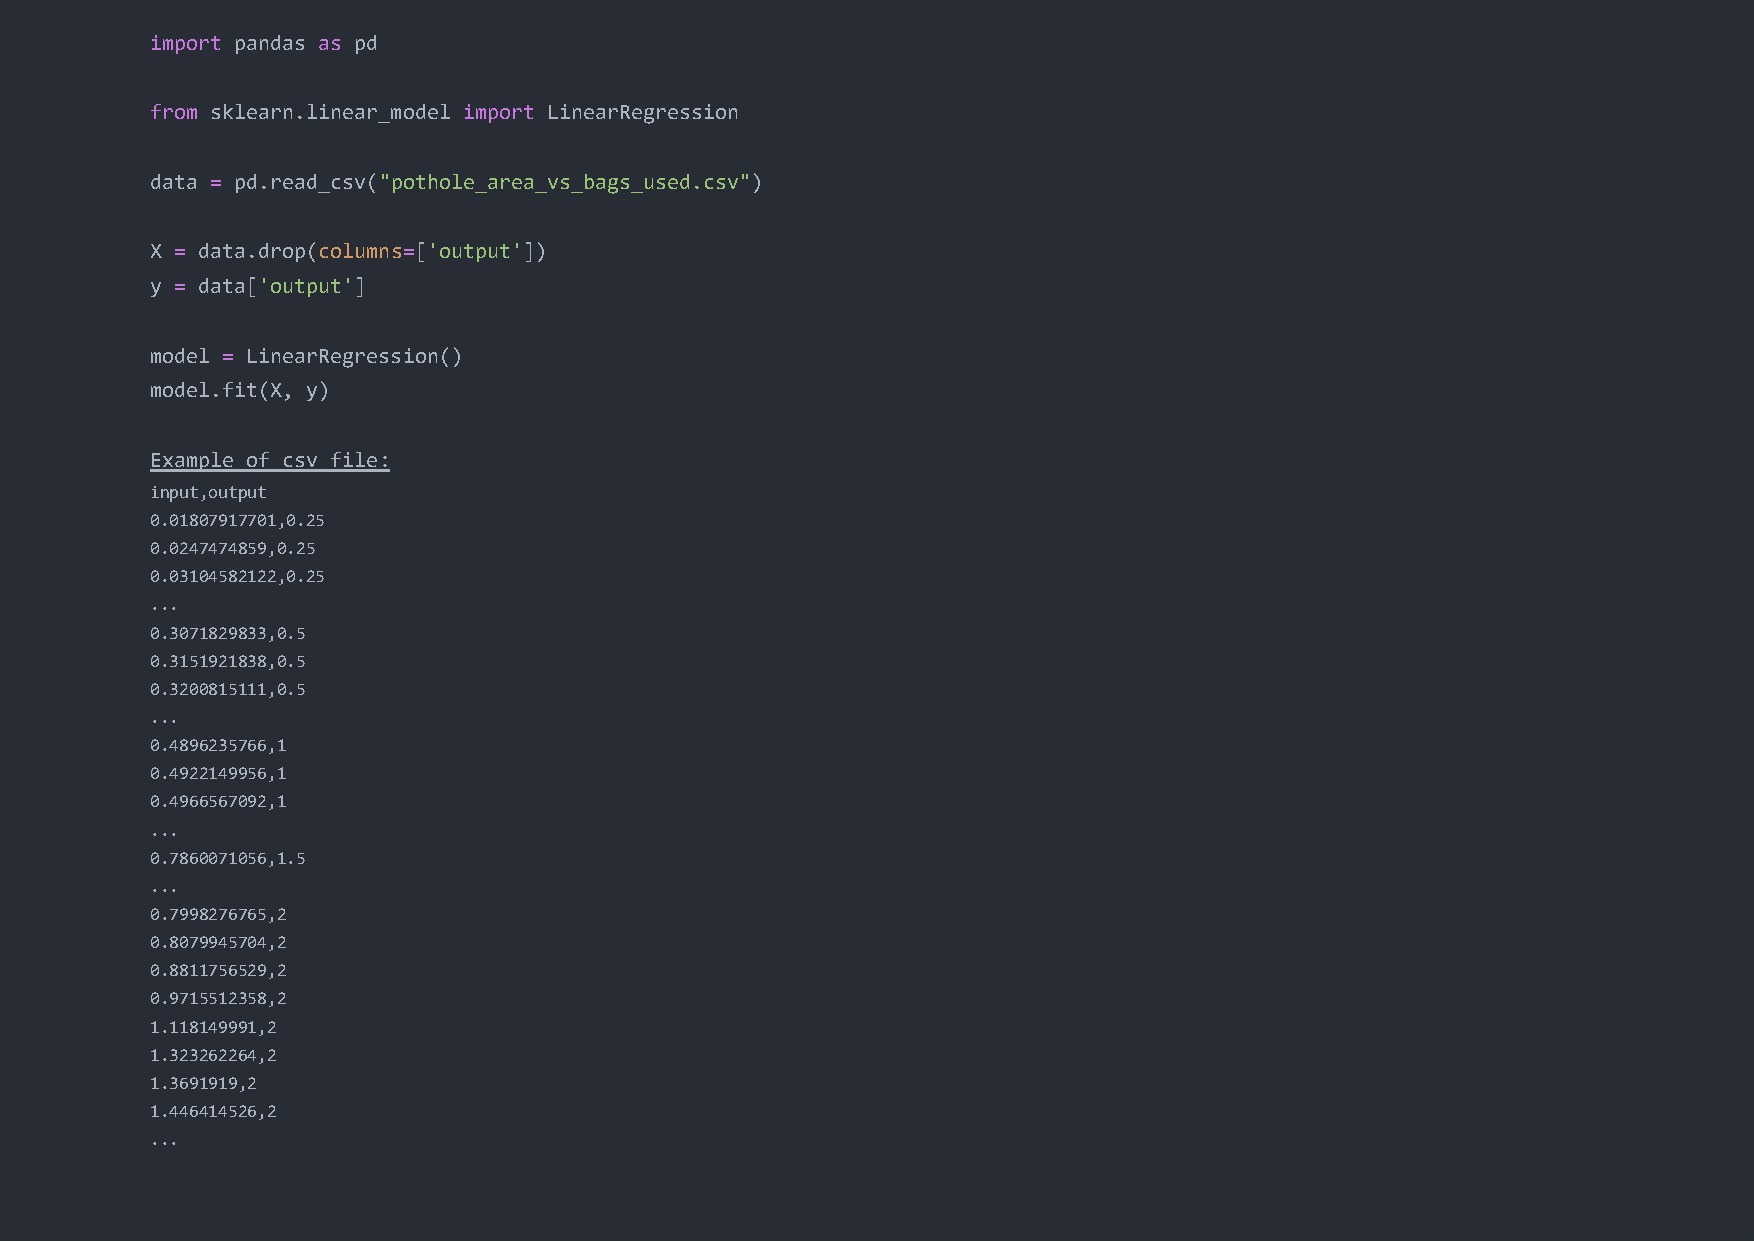
\includegraphics[width=0.50\columnwidth]{learn_linear_code.pdf}
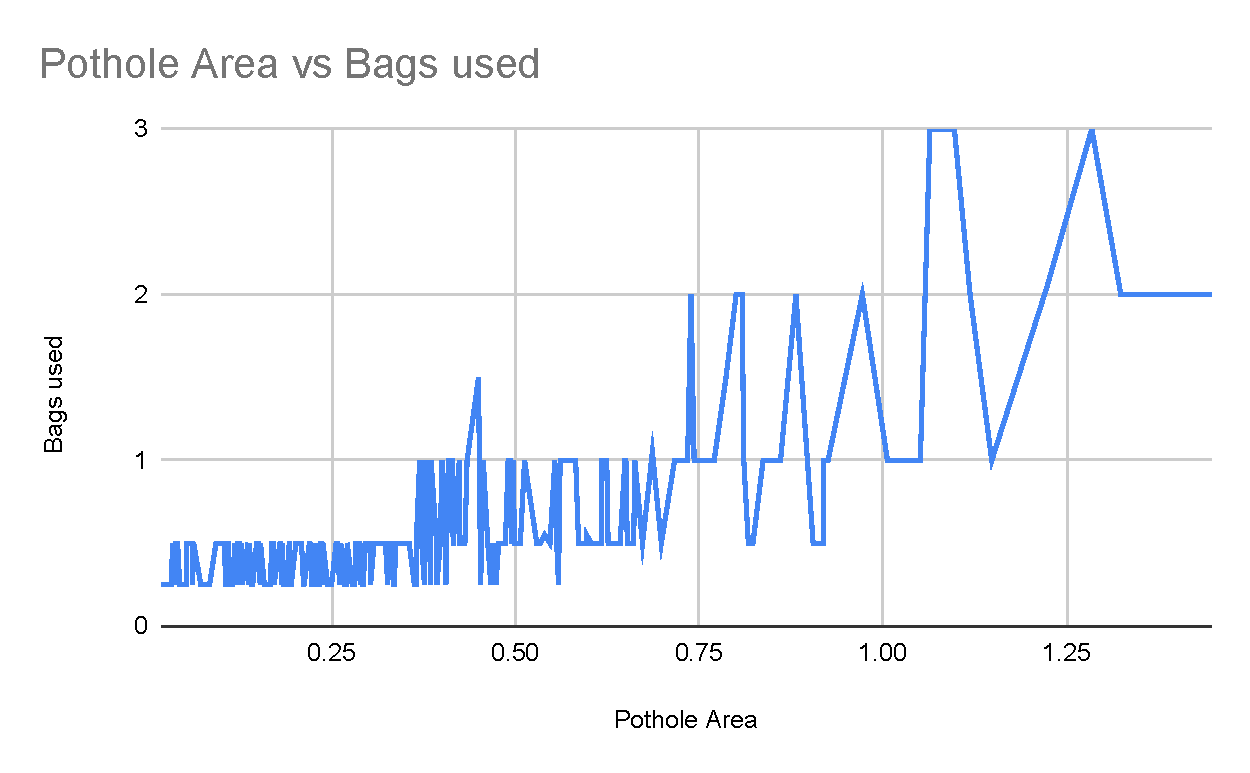
\includegraphics[width=0.50\columnwidth]{sheets_plot.pdf}

\end{document}
